\documentclass[10pt,a4paper,headsepline,smallheadings]{scrartcl}
\usepackage[utf8]{inputenc}
\usepackage[T1]{fontenc}
\usepackage[ngerman]{babel}
\usepackage{amsmath}
\usepackage{amsthm}
\usepackage{amssymb}
\usepackage{amsfonts}
\usepackage[scaled]{helvet}
\usepackage{amssymb}
\usepackage{multirow}
\usepackage{textcomp}
\usepackage{graphicx}
\usepackage{paralist}
\usepackage{textcomp}
\usepackage{pdflscape} 
\usepackage{marvosym}
\usepackage{float}
\usepackage{siunitx}
\usepackage[siunitx,european,cuteinductors,smartlabels]{circuitikz}
\usepackage{fancyhdr}
\usepackage{pgfplots}
\usepackage{sansmath}

\usetikzlibrary{calc}


\theoremstyle{definition}
\newtheorem{aufgabe}{Aufgabe}


\renewcommand*\familydefault{\sfdefault}
\renewcommand{\arraystretch}{1.1}


\KOMAoptions{parskip=half,DIV=15,fontsize=11pt}
\unitlength1cm
\titlehead{

\begin{center}\begin{tabular}{p{10cm}p{6.8cm}}
\textbf{FH Aachen} & \textbf{FB Maschinenbau und Mechatronik}\\[0.5cm]
\textbf{Modul 86111} &  Prof. Dr. Raphael Pfaff\\
Schienenfahrzeugtechnik I& Sommersemester 2015\\
\end{tabular}

\end{center}
\begin{picture}(0,0)(0,0)\put(17,-23){
\includegraphics[height=5cm]{fh_logo}}\end{picture}
}
\newif\ifuelsg %als slides
%\uelsgtrue
\uelsgfalse
\newif\ifnotuelsg
\ifuelsg\notuelsgfalse\else\notuelsgtrue\fi
\graphicspath{
{../Bilder/Uebungen/}
{../Bilder/Wirkungsplan/}
}

%\titlehead{83105 \hfill Mess-Steuerungs- und Regelungstechnik \hfill Prof. Manfred Enning}
\title{Schienenfahrzeugtechnik I  -- \"Ubung 1}
\date{}
\makeatletter
\let\Title\@title
\let\Author\@author
\makeatother
\pagestyle{fancy}
\fancyhead[LE, LO]{Prof. Dr. Raphael Pfaff}
\fancyhead[RE, RO]{\Title}

\begin{document}
\thispagestyle{empty}
\maketitle
\vspace{-2cm}
% \hyphenation{Abwei-chungen}

\section*{Einf\"uhrung in die Zugdynamik}
\begin{aufgabe}[Zugkraftkennlinie] 
Tragen Sie qualitativ die L\"angskr\"afte der unten gezeigte Z\"uge ein.
\begin{center}
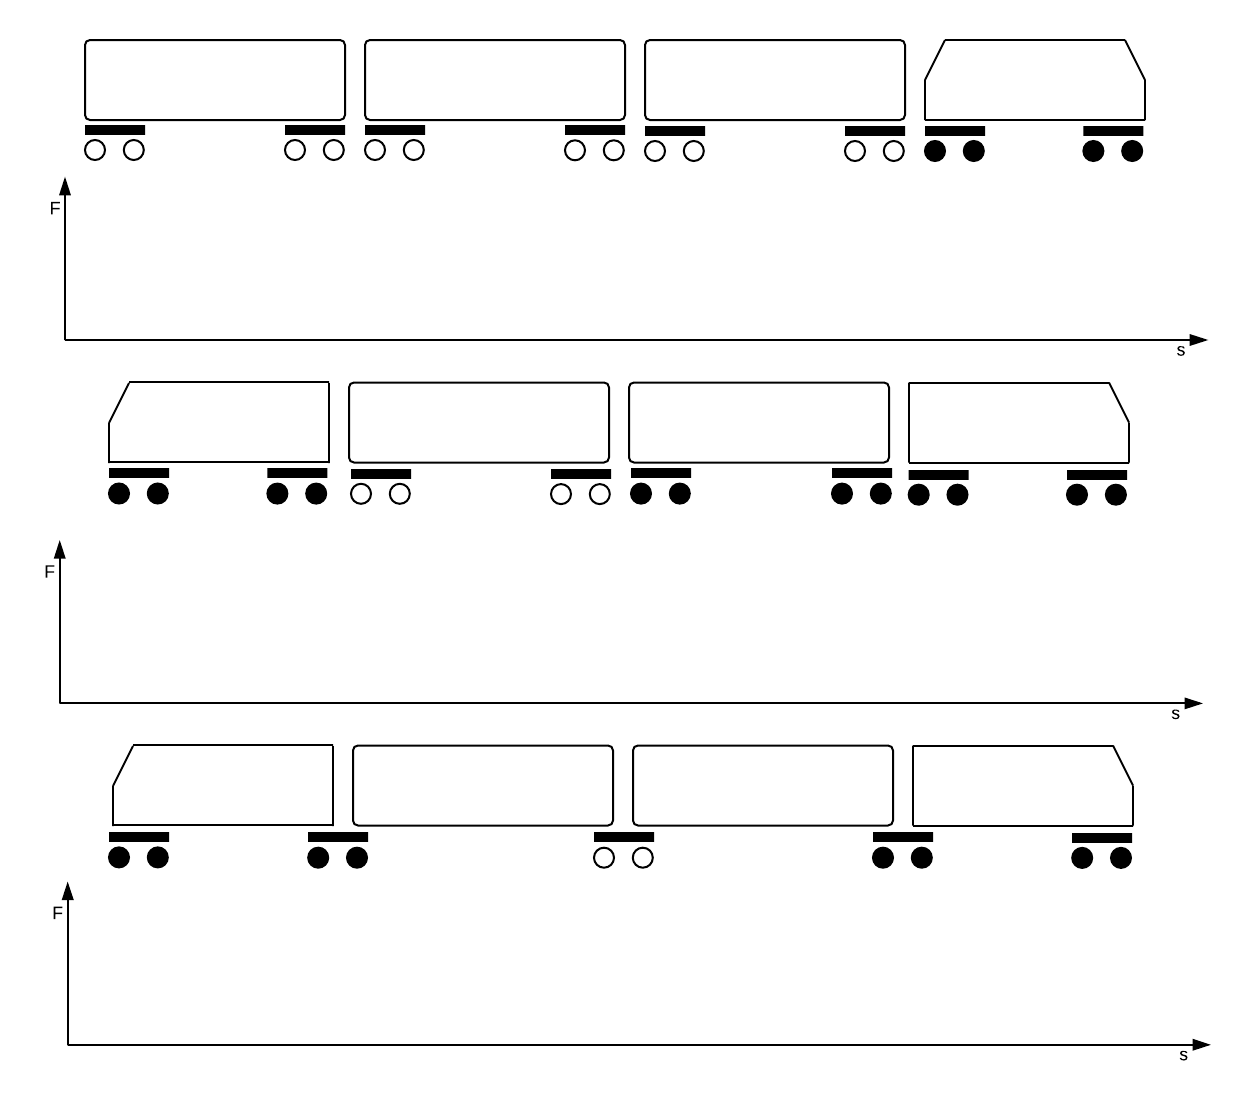
\includegraphics[width = .95\textwidth]{Laengskraefte}
\end{center}
\end{aufgabe}

\begin{aufgabe}[Zugkraftkennlinie] 
Eine Lokomotive der BR 143 der DB AG zieht einen Wagenzug. Die technischen Daten der Fahrzeuge sind:
\begin{itemize}
	\item Triebfahrzeug:
	\begin{itemize}
		\item Masse $m_{L} = 82\, \mathrm{ t}$
		\item Rotierende Masse $m_{DL} = 16\, \mathrm{ t}$
	\end{itemize}
	\item Wagenzug:
	\begin{itemize}
		\item Masse $m_{W} = 500\, \mathrm{t}$
		\item Rotierende Masse $m_{DW} = 24\, \mathrm{t}$
	\end{itemize}
\end{itemize}

\pgfplotsset{width=10 cm}
\begin{center}
	\begin{tikzpicture}
		\begin{axis}[ylabel={$F_{T}/kN$},
		xlabel = {$v/ms^{-1}$}
		%legend, %style={at={(1.5,1)}},
		%anchor=north, legend columns=3},
		%xtick=data
		]]
		\addplot coordinates
			{(0,244) (2.78, 223) (5.55,207) (8.33, 196) (11.11, 189) (13.89, 183) (16.67, 178) (19.44, 174) (22.22, 170) (25, 168) (26.11, 167) (27.78, 144) (29.17, 129) (30.56, 117) (31.94, 107) (33.33, 100)};
			\addplot coordinates
			{(0,11.2) (2.78, 11.5) (5.55, 12.5) (8.33, 13.3) (11.11, 14.8) (13.89, 16.7) (16.67, 18.9) (19.44, 21.6) (22.22, 24.6) (25, 28) (26.11,29.4 ) (27.78, 31.7) (29.17, 33.8) (30.56, 35.9) (31.94, 38.1) (33.33, 40.5)};
			%\addplot coordinates %2%-Gefaelle
			%{(0,111.2) (2.78, 111.5) (5.55, 112.5) (8.33, 113.3) (11.11, 114.8) (13.89, 116.7) (16.67, 118.9) (19.44, 121.6) (22.22, 124.6) (25, 128) (26.11,129.4 ) (27.78, 131.7) (29.17, 133.8) (30.56, 135.9) (31.94, 138.1) (33.33, 140.5)};
		\legend{$F_{T}(v)$, $F_{WZ}(v)$};
		\end{axis}
\end{tikzpicture}
\end{center}

\begin{enumerate}[a)]
\item Zeichnen Sie die Widerstandskurven des Zugverbands (bestehend aus Lokomotive und Wagenzug) f\"ur Streckenneigungen $i_{k} = (1, 2, 4) \%$ in das $F-v$-Diagramm ein. Der Fahrwiderstand des Triebfahrzeugs ist zu vernachl\"assigen.
\item Bestimmen Sie die H\"ochstgeschwindigkeiten $v_{max, k}$ in den jeweiligen Streckenneigungen.
\item Bestimmen Sie das Beschleunigungsverm\"ogen des Zugverbands in der Ebene und in 1\% Streckenneigung f\"ur $v = 90\, \mathrm{km/h}$.
\item Bestimmen Sie die kinetische Energie des Zugverbands bei $v = 120 \, \mathrm{km/h}$ und bestimmen Sie f\"ur einen mittleren Fahrwiderstand von $F_{W,m} =20 \, \mathrm{kN}$ in einer Steigung von 1\% die Steigh\"ohe bis v = 0 gilt.
\end{enumerate}
\end{aufgabe}

\end{document}